\chapter{Code Migration}
\section{Cosa è?}
La code migration consiste nel trasferimento di un programma (o di una sua parte) da una macchian a l'altra.

Il codice può può essere trasferito:
\begin{itemize}
    \item Prima dell'esecuzione
    \item Durante l'esecuzione, con migrazione dello stato
\end{itemize}

Questo fa diventare il codice una enitità mobile all'interno del sistema distribuito, permettendo cosi'di ottimizzare le prestanzioni nei seguenti modi:
\begin{itemize}
    \item Spostare i processi da macchine sovraccariche a macchine scariche (load distribution)
    \item Minimizzare la comunicazione spostando il calcolo dove risiedono i dati
    \item Evitare il trasferimento di grandi moldi di dati grazzi attraverso la rete
\end{itemize}

\section{Flessibilità}
Nello sviluppo classico di applicazioni distributi si decide a priori dove ciascun componente deve essere eseguito.

Se invece il codice può spostarsi tra le macchine:
\begin{itemize}
    \item Il sistema distribuito può essere configurato dinamicamente
    \item Le funzionalità possono essere installate solo quando servono
    \item Il binding client-server diventà più flessibile
\end{itemize}

\begin{figure}[H]
    \centering
    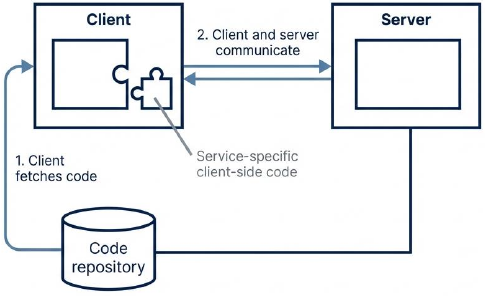
\includegraphics[scale=0.5]{figures/Schermata_20260603_122616.png}
\end{figure}

\section{Sicurezza}
Il problema principale è la sicurezza:
\begin{itemize}
    \item Il codice scaricato potrebbe essere malevolo
    \item Potrebbe accedere a risorse locali
    \item Potrebbe esfiltrare dati
\end{itemize}

\section{Tipi di mobilità}
\subsection{Modalità debole}
Nella modalità debole si trasferisce solo il code segment: il programma riparte sempre dall'inizio sulla destinazione.

\begin{figure}[H]
    \centering
    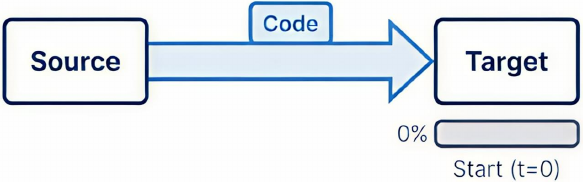
\includegraphics[scale=0.65]{figures/Schermata_20260603_123107.png}
\end{figure}

Esistono due varianti che differiscono per chi prende l'iniziativa:
\begin{itemize}
    \item \textbf{REV (Remote Evaluation)}

    Il client invia il proprio codice al server perchè lo esegue usando le risorse del server.

    \begin{figure}[H]
        \centering
        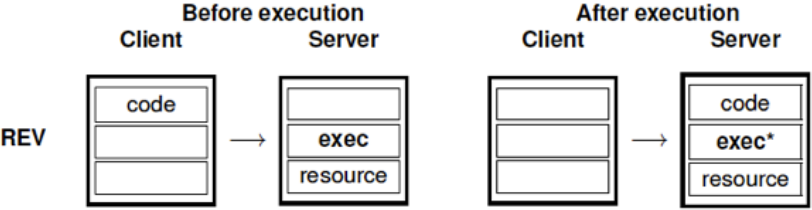
\includegraphics[scale=0.6]{figures/Schermata_20260603_123322.png}
    \end{figure}
    
    \item \textbf{CoD (Code on Demand)}

    Il client scarica codice dal server per eseguirlo localmente

    \begin{figure}[H]
        \centering
        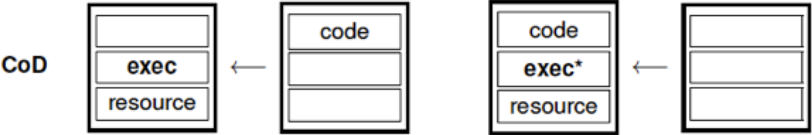
\includegraphics[scale=0.6]{figures/Schermata_20260603_123441.png}
    \end{figure}
\end{itemize}

\newpage
\subsection{Strong mobility}
Si trasferiscono codice e segmentano di esecuzione, il processo riprende sulla destinazione esattamente nello stato in cui era stato sospeso.

\begin{figure}[H]
    \centering
    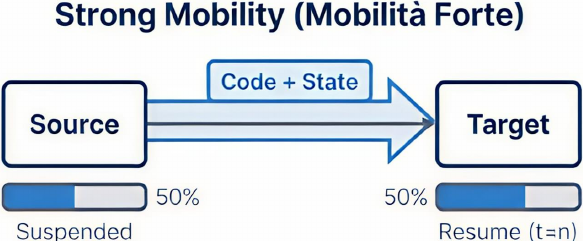
\includegraphics[scale=0.65]{figures/Schermata_20260603_125239.png}
\end{figure}

\section{Problema dell'eterogeneità}
\begin{figure}[H]
    \centering
    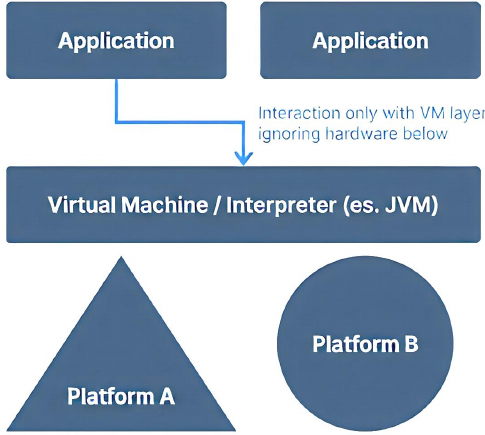
\includegraphics[scale=0.65]{figures/Schermata_20260603_125619.png}
\end{figure}
\subsection{Remote Evaluation (REV)}
\begin{itemize}
    \item Il client invia il codice al server per l'esecuzione
    \item Sfrutta le risorse del server
    \item Esempio: invio di uno script di ricerca a un database remoto
    \item Modifica lo stato di esecuzione sul server
\end{itemize}
\subsection{Code on Demand (CoD)}
\begin{itemize}
    \item Il client richiede e scarica il codice del server
    \item Sfrutta le risorse locali del client
    \item Vantaggio: maggiore flessibilità e prestazioni, senza installazione permanente
\end{itemize}

\chapter{Applicazioni Data-Intensive}
\section{Cosa sono?}
Sono applicazioni il cui collo di bottiglia non è la potenz di calcolo, ma il volume, la velocità e la varietà dei dati da elaborare.

Sono caratterizzate dalle \textbf{3 V}:
\begin{itemize}
    \item \textbf{Volume}: TB/PB di dati che non stanno su una singola macchina
    \item \textbf{Velocity}: Dati prodotti e da analizzare in tempo realo o quasi reale
    \item \textbf{Variety}: Formati eterogenei, da tabelle relazionali a log, immagini, testo, JSON
\end{itemize}

\begin{figure}[H]
    \centering
    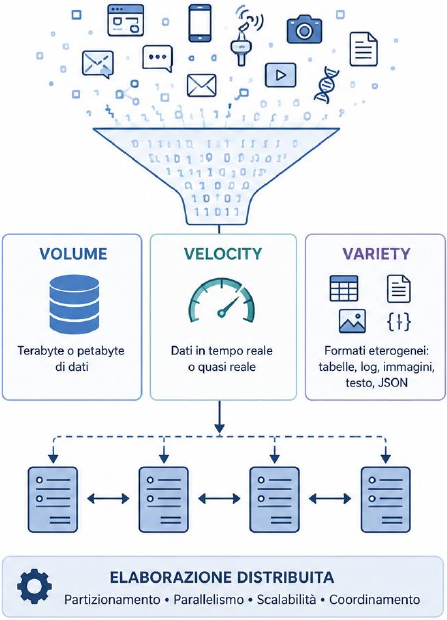
\includegraphics[scale=0.77]{figures/Schermata_20260603_130906.png}
\end{figure}

\section{L'idea: portare la computazione vicino ai dati}
Una computazione richesta da un'applicazione è molto più efficiente se viene eseguita vicino ai dati.

Questo è particolarmente vero quando la dimensione del dataset è enorme.

Questo minimizza la congestione di rete aumenta il complessivo throughtput del sistema

\begin{figure}[H]
    \centering
    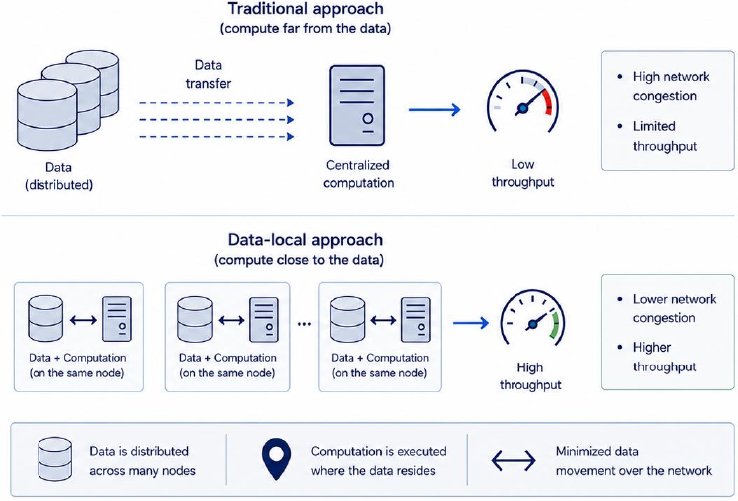
\includegraphics[scale=0.8]{figures/Schermata_20260603_131229.png}
\end{figure}

\newpage
\section{Le 3 dimensioni della scalabilità}
\begin{itemize}
    \item \textbf{Scalabilità Dimensionale}: Capacità di aggiungere facilmente più utenti e risorse senza degradare le prestazioni.
    \item \textbf{Scalabilità Geografica}: Capacità del sistema di gestire utenti e risorse situati a grandi distanze, rendendo i ritardi di comunicazione (latenza) quasi impercettibili
    \item \textbf{Scalabilità Amministrativa}: Capacità di gestire il sistema anche quando si estende su diverse organizzazioni indipendenti con politichè differenti
\end{itemize}

\begin{figure}[H]
    \centering
    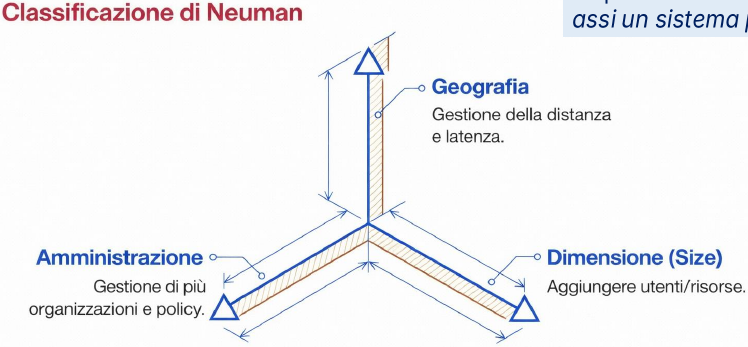
\includegraphics[scale=0.65]{figures/Schermata_20260603_131608.png}
\end{figure}

\subsection{Scale Cube}
\begin{figure}[H]
    \centering
    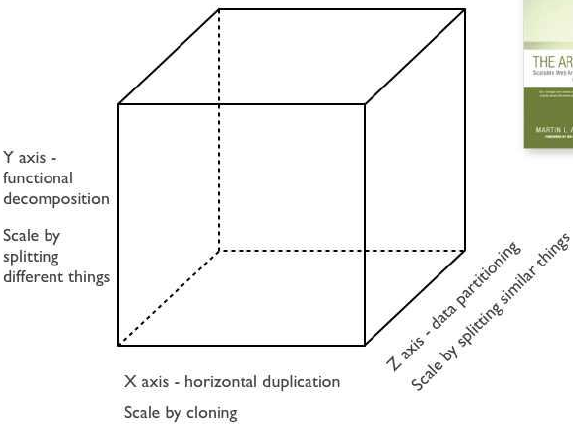
\includegraphics[scale=0.66]{figures/Schermata_20260603_152206.png}
\end{figure}
\begin{itemize}
    \item \textbf{Asse X}: Replicazione - eseguire più istanze di un applicazione dietro un load balancer
    \item \textbf{Asse Y}: Decomposizione funzionale - suddivisione dell'applicazione in più servizi distinti
    \item \textbf{Asse Z}: Partizionamento dei dati - ogni server è responsabile solo di un sottoinsieme di dei dati
\end{itemize}